\documentclass[11pt]{amsart}
\usepackage{geometry}                % See geometry.pdf to learn the layout options. There are lots.
\geometry{letterpaper}                   % ... or a4paper or a5paper or ... 
%\geometry{landscape}                % Activate for for rotated page geometry
%\usepackage[parfill]{parskip}    % Activate to begin paragraphs with an empty line rather than an indent
\usepackage{graphicx}
\usepackage{amssymb}
\usepackage{epstopdf}
\DeclareGraphicsRule{.tif}{png}{.png}{`convert #1 `dirname #1`/`basename #1 .tif`.png}
% listings
\usepackage{listings}
\usepackage{color}
%
%
\begin{document}
% document options
\title{ENAPP 2012 - Webshop}
\author{Iwan Paolucci}
%
\maketitle
%
%\newpage{}
%%%%%%%%%%%%%%%%%%%%%%%%%%%%%%%%%
% Introduction
%%%%%%%%%%%%%%%%%%%%%%%%%%%%%%%%%
\section{Intro}
In the module ENAPP.H12 a Webshop has to be developed. This documentation covers the most neccesary information and a short overview of the architecture. \\
\subsection{}Technology\\
A short overview over the technologies used.
\begin{itemize}
\item J2EE 1.6 (Java Enterprise Edition)
\item Java 7
\item Java Server Faces (JSF)
\item Java Message Service (JMS)
\item SOAP Webservices
\item Rest Webservices
\item JDBC / JPA (MySQL)
\end{itemize}
%
\subsection{}Usage\\
The application is more or less self-explanatory or should be. There are seperate users for administration and shopping. A already installed user can be used or a new one can be created. \\
%
\textbf{Webshop}\\
\textsf{0160.intra015.el.campus.intern:8080/enapp12-tapaoluc-web/index.xhtml} \\
User/Password: dude/dude\\
%
\textbf{Adminpanel} \\
\textsf{0160.intra015.el.campus.intern:8080/enapp12-tapaoluc-web-admin/index.xhtml} \\
User/Password: admin/admin \\
\newpage{}
%%%%%%%%%%%%%%%%%%%%%%%%%%%%%%%%%
% Infrastructure
%%%%%%%%%%%%%%%%%%%%%%%%%%%%%%%%%
\section{Infrastructure} 
%
This section covers information about the Infrastructure. \\
%\subsection{}Development \\
%\textbf{Database} \\
%User: root \\
%Password: 123 \\
% 
\subsection{}Integration \\
Description of the integrationplattform in the EnterpriseLab @ HSLU.\\
\subsubsection{}OperatingSystem \\
Type: Solaris \\
User: tapaoluc (EL User) \\
root Password: ENAPP\_H12
%
\subsubsection{}Database \\
Type: MySQL \\
Server: s0160.intra015.el.campus.intern \\
User: enapp \\
Password: enapp 
%
\subsubsection{}Applicationserver \\
Type: Glassfish 3+ \\
Adminpanel: https://s0160.intra015.el.campus.intern:4848 \\
User: admin \\
Password: ENAPP\_H12 \\
%
\subsubsection{}/etc/hosts \\
For the connection to the Navision service an additional entry to the hosts file is needed.\
\begin{verbatim}
#navision
10.29.2.12      icompanydb01.icompany.intern
\end{verbatim}
%
\subsection{Configuration}
\subsubsection{}Database \\
\textit{JDBC Connection Pool}\\
Poolname: EnappWebshopTapaolucPool \\
Resource Type: javax.sql.DataBase \\
Datasource Classname: com.mysql.jdbc.jdbc2.optional.MysqlDataSource \\
% additional
\textit{Additional Properties on Connection Pool} \\
password = enapp \\
user = enapp \\
servername = s0160.intra015.el.campus.intern \\
roleName = com.mysql.jdbc.Driver \\
datasourceName = jdbc:mysql://s0160.intra015.el.campus.intern:3306/enappwebshop \\
databaseName = enappwebshop \\
portNumber = 3306 \\
%
\textit{Ressource} \\
JNDI Name: jdbc/enappwebshoptapaoluc \\
Poolname: EnappWebshopTapaolucPool \\
%
\subsubsection{}Java Message Service \\
\textit{Queuefactory} \\
Poolname: jms/purchasequeuefactory \\
Ressource Type: javax.jms.QueueConnectionFactory \\
Transaction: XATransaction \\
AdditionalProperty: AddressList = mq://10.29.3.152:7676/jms \\
\textit{Queue} \\
JNDI Name: jms/purchasequeue \\
Physical Name: EnappQueue \\
Resource Type: javax.jms.Queue \\
%
\subsubsection{}Security
%
\textit{Security - Realm} \\
Configuration: server-config \\
Realm Name: enappwebshoprealm \\
Classname: com.sun.enterprise.security.auth.realm.jdbc.JDBCRealm \\
JAAS Context: jdbcRealm \\
JNDI Name: jdbc/enappwebshoptapaoluc \\
Usertable: customer \\
Usercolumn: username \\
Passwordcolumn: password \\
Grouptable: customergroups \\
Grouptable-Usercolumn: username \\
Groupcolumn: groupname \\
Digest algorithm: none \\
Encryption algorithm: none \\
%
\textbf{Attention: There is no encryption so do not use your own passwords for tests!}
%
\subsubsection{}JNDI - Custom Ressources \\
This setting sets the stage of the application to production. \\
JNDI Name: javax.faces.PROJECT\_STAGE \\
Ressource Type: java.lang.String \\
Factory Class: org.glassfish.resources.custom.factory.PrimitivesAndStringFactory \\
Property: stage = production \\
%
\newpage{}
%%%%%%%%%%%%%%%%%%%%%%%%%%%%%%%%%
% Architectural overview
%%%%%%%%%%%%%%%%%%%%%%%%%%%%%%%%%
\section{Architecture}
Below is an overview of the webshop. It is a component based architecture. All accesses to other components are done via Interfaces defined in \textsf{enapp12-tapaoluc-lib}. The general idea of this architecture is to avoid any changes in business logic when the datasource changes. For example when the purchase is sent to a JMS queue insted of stored in a relational database, in general there shouldn't be any changes insted of some annotations tellig CDI that another implementation is needed.\\
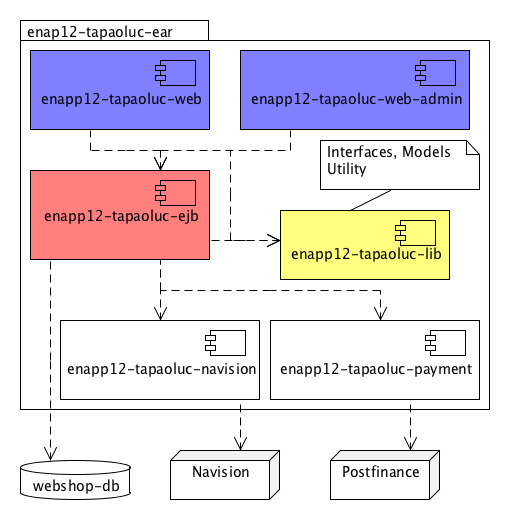
\includegraphics[scale=0.8]{component-dia.png}\\
Inside the EJB component a "Entity Controller Boundary" pattern is implemented. Below there is a sample from the Purchase. \\
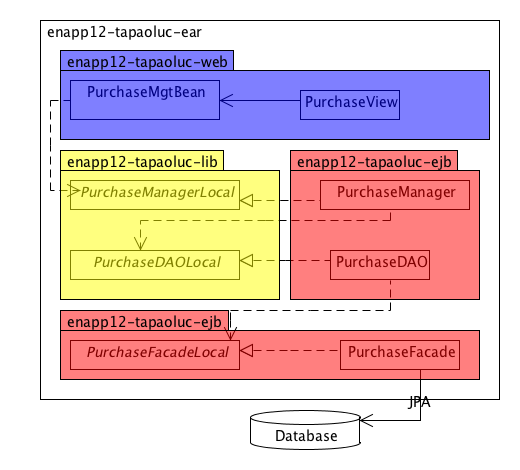
\includegraphics[scale=0.8]{sample-arch.png}\\
The JSF Managed Bean accesses the PurchaseManager via the Interface PurchaseManagerLocal. The PurchaseManager has the BusinessLogic implemented and gets hist Data from PurchaseDAO via PurchaseDAOLocal. The implementations are injected via the Context and Dependency Injection. 
\newpage{}
In code it looks like this (this ist not the actual code but it shows the general idea):\\
\begin{lstlisting}
/* PurchaseMgmtBean.java (web)*/
@Inject
private PurchaseManagerLocal pml;

public void checkoutPurchase(){
	// collect data entered from user and send it to ejb
	this.pml.checkoutPurchase(purchase);
}


/* PurchaseManager.java (ejb)*/
@Inject
@JMSPurchaseDAO
private PurchaseDAOLocal dao;

@Inject
@PostfinancePayment
private CreditCardPayment payment;

private boolean anythingWentWrong;

public void checkoutPurchase(Purchase purchase){
	// do the payment
	payment.pay();
	// store purchase
	dao.storePurchase(purchase);
	// send feedback if neccesary
	if(anythingWentWrong){
		throw new BusinessException("something wrong");
	}
}


/* PurchaseDAO (JMS impl) */
@StatelessBean
@JMSPurchaseDAO
public class JMSPurchaseDataAccess implements PurchaseDAOLocal{}
\end{lstlisting}
\lstset{language=Java,caption={CDI},label=CDI} 
%
When the Interface to the Purchase service changes for example to a Rest service there is only the Annotation \textsf{@JMSPurchaseDAO} changed to \textsf{@RestPurchaseDAO} which points to the Rest implemenation. \\
\subsection{}Project Structure \\
Below the structure of the project is visualized. At the end everything is packed into one EAR (Enterprise Archtive). In the \textsf{enapp12-tapaoluc-lib} project in packages boundary and dataaccess are only interfaces not implementations.\\
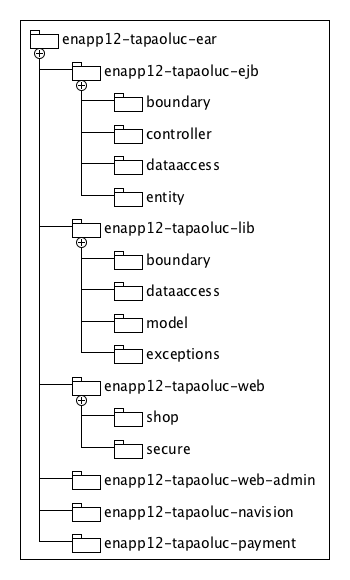
\includegraphics[scale=0.7]{project-structure.png}
\end{document}